\noindent\textbf{Solution 1 } \\\\

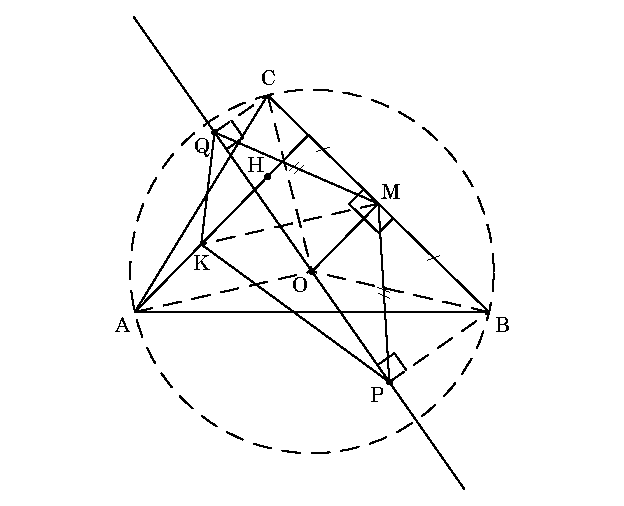
\includegraphics{share/euk/51M04_rmm202300004_1.eps}

Por los datos del enunciado del problema

\begin{equation} \label{eq_51M04_rmm202300004_1}
	triangle(A, B, C)
\end{equation}
\begin{equation} \label{eq_51M04_rmm202300004_2}
	\angle{ABC} < \ang{90} \land \angle{BCA} < \ang{90} \land \angle{CAB} < \ang{90}
\end{equation}
\begin{equation} \label{eq_51M04_rmm202300004_3}
	circle(\sigma) \land \forall X \i \{A, B, C\}\ X \in \sigma
\end{equation}
\begin{equation} \label{eq_51M04_rmm202300004_4}
	O = center(\sigma)
\end{equation}
\begin{equation} \label{eq_51M04_rmm202300004_5}
	{AH \perp BC} \land {BH \perp AC} \land {CH \perp AB}
\end{equation}
\begin{equation} \label{eq_51M04_rmm202300004_6}
	K \in \overline{AH} \land \mid\overline{AK}\mid = \mid\overline{KH}\mid
\end{equation}
\begin{equation} \label{eq_51M04_rmm202300004_7}
	line(\ell) \land O \in \ell
\end{equation}
\begin{equation} \label{eq_51M04_rmm202300004_8}
	P \in \ell \ \ell \perp BP
\end{equation}
\begin{equation} \label{eq_51M04_rmm202300004_9}
	Q \in \ell \ \ell \perp CQ
\end{equation}

Sea $M$ el punto medio de $BC$. 

\begin{equation} \label{eq_51M04_rmm202300004_10}
	M \in \overline{BC}\ \mid\overline{BM}\mid = \mid\overline{MC}\mid
\end{equation}

\begin{claim}
	Los cuadriláteros $OMCQ$ y $OMBP$ son cíclicos.
\end{claim}
\textit{Proof}
\begin{equation} \label{eq_51M04_rmm202300004_11}
	\labelcref{eq_51M04_rmm202300004_3}, \labelcref{eq_51M04_rmm202300004_4}, \labelcref{eq_51M04_rmm202300004_11} \vdash OM \perp BC
\end{equation}
\begin{equation} \label{eq_51M04_rmm202300004_12}
	\labelcref{eq_51M04_rmm202300004_11}, \labelcref{eq_51M04_rmm202300004_8} \vdash \exists \sigma_P\ circle(\sigma_P) \land \forall X \in \{O, M, B, P\}\ X \in \sigma_P
\end{equation}
\begin{equation} \label{eq_51M04_rmm202300004_13}
	\labelcref{eq_51M04_rmm202300004_11}, \labelcref{eq_51M04_rmm202300004_9} \vdash \exists \sigma_Q\ circle(\sigma_Q) \land \forall X \in \{O, M, C, Q\}\ X \in \sigma_Q
\end{equation}
\hfill $\square$

\begin{claim}
	Los $\triangle{OBC}$ y $\triangle{MPQ}$ son semejantes.
\end{claim}
\textit{Proof}
\begin{equation} \label{eq_51M04_rmm202300004_14}
	\labelcref{eq_51M04_rmm202300004_12} \vdash \angle{OBC} = \angle{MPO}
\end{equation}
\begin{equation} \label{eq_51M04_rmm202300004_15}
	\labelcref{eq_51M04_rmm202300004_13} \vdash \angle{OCB} = \angle{MQO}
\end{equation}
\begin{equation} \label{eq_51M04_rmm202300004_16}
	\labelcref{eq_51M04_rmm202300004_14}, \labelcref{eq_51M04_rmm202300004_15}, \labelcref{eq_51M04_rmm202300004_7}, \labelcref{eq_51M04_rmm202300004_8}, \labelcref{eq_51M04_rmm202300004_9} \vdash \triangle{OBC} \sim \triangle{MPQ}
\end{equation}
\hfill $\square$

Como consecuencia

\begin{equation} \label{eq_51M04_rmm202300004_16a}
	\labelcref{eq_51M04_rmm202300004_16} \vdash \frac{\mid\overline{PQ}\mid}{\mid\overline{PM}\mid} =\frac{\mid\overline{BC}\mid }{\mid\overline{OB}\mid }
\end{equation}

\begin{equation} \label{eq_51M04_rmm202300004_17}
	\labelcref{eq_51M04_rmm202300004_3}, \labelcref{eq_51M04_rmm202300004_4} \vdash \mid\overline{OA}\mid = \mid\overline{OB}\mid = \mid\overline{OC}\mid 
\end{equation}
\begin{equation} \label{eq_51M04_rmm202300004_18}
	\labelcref{eq_51M04_rmm202300004_16}, \labelcref{eq_51M04_rmm202300004_17} \vdash \mid\overline{MP}\mid = \mid\overline{MQ}\mid
\end{equation}

Recurriendo al siguiente teorema conocido.

\begin{theorem} \label{th_51M04_h2v_2x_o2m}
	La distancia del ortocentro a un vértice es el doble de la distancia del circuncentro al (punto medio del) lado opuesto.
	\begin{equation}
	\begin{gathered}
		triangle(A,B,C) \land (AH \perp BC) \land (BH \perp AC) \land (CH \perp AB) \land \\
		circle(\sigma) \land \forall X \in \{A,B,C\}\ X \in \sigma \land O = center(\sigma) \\
		(M \in \overline{BC}\ \mid\overline{BM}\mid = \mid\overline{MC}\mid) \vdash \mid\overline{AH}\mid = 2 \cdot \mid\overline{OM}\mid
	\end{gathered}
	\end{equation}
\end{theorem}

\begin{claim}
	Se cumple que $\mid\overline{KM}\mid = \mid\overline{OA}\mid$
\end{claim}
\textit{Proof}
\begin{equation} \label{eq_51M04_rmm202300004_19}
	\cref{th_51M04_h2v_2x_o2m},\labelcref{eq_51M04_rmm202300004_1}, \labelcref{eq_51M04_rmm202300004_6}, \labelcref{eq_51M04_rmm202300004_3}, \labelcref{eq_51M04_rmm202300004_4}, , \labelcref{eq_51M04_rmm202300004_10} \vdash \mid\overline{HA}\mid =  2 \cdot \mid\overline{OM}\mid
\end{equation}
\begin{equation} \label{eq_51M04_rmm202300004_20}
	\labelcref{eq_51M04_rmm202300004_19}, \labelcref{eq_51M04_rmm202300004_6} \vdash \mid\overline{KA}\mid = \mid\overline{OM}\mid
\end{equation}
\begin{equation} \label{eq_51M04_rmm202300004_21}
	\labelcref{eq_51M04_rmm202300004_5}, \labelcref{eq_51M04_rmm202300004_11} \vdash OM \parallel AH
\end{equation}

Por lo tanto $AOMK$ es un paralelogramo, y por consiguiente

\begin{equation} \label{eq_51M04_rmm202300004_22}
	\labelcref{eq_51M04_rmm202300004_20}, \labelcref{eq_51M04_rmm202300004_21} \vdash (AO \parallel KM) \land (\mid\overline{AO}\mid = \mid\overline{KM}\mid)
\end{equation}
\hfill $\square$

Finalmente recurramos al siguiente resultado conocido

\begin{theorem} \label{th_51M04_ptolomeys_ineq} \textbf{Desigualdad de Ptolomeo}
	Sea $ABCD$ un cuadrilátero siempre se cumple que 
	\begin{equation} \label{eq_th_51M04_ptolomeys_ineq_1}
		\mid\overline{AB}\mid \cdot \mid\overline{CD}\mid + \mid\overline{BC}\mid \cdot \mid\overline{AD}\mid \geq \mid\overline{AC}\mid \cdot \mid\overline{BD}\mid
	\end{equation}
	El caso de igualdad sucede si, y solamente si, $ABCD$ es cíclico.
	\begin{equation} \label{eq_th_51M04_ptolomeys_ineq_2}
		\mid\overline{AB}\mid \cdot \mid\overline{CD}\mid + \mid\overline{BC}\mid \cdot \mid\overline{AD}\mid = \mid\overline{AC}\mid \cdot \mid\overline{BD}\mid \leftrightarrow \exists \sigma\ circle(\sigma) \land \forall X \in \{A,B,C,D\} X \in \sigma
	\end{equation}
\end{theorem}

... y aplicándolo al cuadrilátero $KPMQ$ ...

\begin{equation} \label{eq_51M04_rmm202300004_23}
	\cref{th_51M04_ptolomeys_ineq} \vdash \mid\overline{KP}\mid \cdot \mid\overline{MQ}\mid + \mid\overline{KQ}\mid \cdot \mid\overline{MP}\mid \geq \mid\overline{KM}\mid \cdot \mid\overline{PQ}\mid
\end{equation}
\begin{equation} \label{eq_51M04_rmm202300004_24}
	\labelcref{eq_51M04_rmc2007dr071_23}, \labelcref{eq_51M04_rmc2007dr071_18} \vdash \mid\overline{KP}\mid + \mid\overline{KQ}\mid \geq \frac{\mid\overline{KM}\mid \cdot \mid\overline{PQ}\mid}{\cdot \mid\overline{PM}\mid }
\end{equation}
\begin{equation} \label{eq_51M04_rmm202300004_25}
	\labelcref{eq_51M04_rmc2007dr071_24}, \labelcref{eq_51M04_rmc2007dr071_16a} \vdash \mid\overline{KP}\mid + \mid\overline{KQ}\mid \geq \frac{\mid\overline{KM}\mid \cdot \mid\overline{BC}\mid}{\cdot \mid\overline{OB}\mid }
\end{equation}
\begin{equation} \label{eq_51M04_rmm202300004_26}
	\labelcref{eq_51M04_rmc2007dr071_25}, \labelcref{eq_51M04_rmc2007dr071_22}, \labelcref{eq_51M04_rmc2007dr071_17} \vdash \mid\overline{KP}\mid + \mid\overline{KQ}\mid \geq \mid\overline{BC}\mid
\end{equation}

\vspace{1cm}
Lo que queda demostrado. \\\\\\
